
\documentclass{article}
\usepackage{geometry}

\geometry{a4paper, margin=0.5cm}
\usepackage[frenchb]{babel}
\usepackage{longtable}
\usepackage{makecell}
\usepackage{xcolor}
\usepackage{hyperref}
\usepackage{graphicx}
\usepackage{multicol}
\definecolor{colorComptoir}{RGB}{253,215,114}
\newcommand{\nameWidth}{13cm}
\newcommand{\dataWidth}{6cm}
\setlength{\footskip}{0pt}
\hypersetup{
    colorlinks=true,
    linkcolor=blue,
    filecolor=magenta,
    urlcolor=cyan,
    }
\begin{document}


  \begin{center}
    
\includegraphics[width=\linewidth]{bandeau_tinda.png}
  \end{center}
\today

    \vspace{.5cm}
    \noindent L’association De Main En Main vous présente l’annuaire des prestataires de la T!nda qui a
vocation à rassembler les acteurs de la transition écologique et sociale en Béarn. Une carte interactive en ligne
    est disponible en plus de cet annuaire (\url{https://carte.demainenmain.org}).
    \vspace{.5cm}

    \noindent La T!nda a pour objectif de soutenir une certaine économie locale, respectueuse des humains et de la nature. La commission prestataire 
    de l'association agrémente les prestataires selon quatre critères :
    \begin{multicols}{2}
    \begin{itemize}
      \item[\textbf{Territoire}]  La relocalisation des échanges économiques est un des enjeux de la monnaie locale. 
        Les informations utilisées pour l'évaluation sont l’emplacement du siège social, la proportion de fournisseurs locaux, le
type de commercialisation ainsi que l’appartenance à une entité telle qu’une coopérative, une autorité de contrôle bio
ou locale.
    \vspace{.2cm}
\item[\textbf{Social}] Les pratiques économiques et sociales des membres du réseau ont de l'importance. Nous nous intéressons donc au statut de
l’entreprise, à l’indépendance du prestataire en matière de décision, à l’échelle des salaires au sein de l’entreprise
et à l’accessibilité de la population aux biens et services proposés.
    \vspace{.2cm}
\item[\textbf{Écologie}] L’activité du prestataire est-elle soucieuse de la préservation de la nature ? Les éléments étudiés pour cette
évaluation sont tous les moyens mis en œuvre pour réduire la consommation énergétique et l’utilisation de produits
chimiques de synthèse.
    \vspace{.2cm}
\item[\textbf{Finance}] À quelle banque adhèrent les prestataires ? Et qu’en est-il de leur participation à l’économie sociale et à la
finance solidaire ?
    \end{itemize}

  \begin{center}
    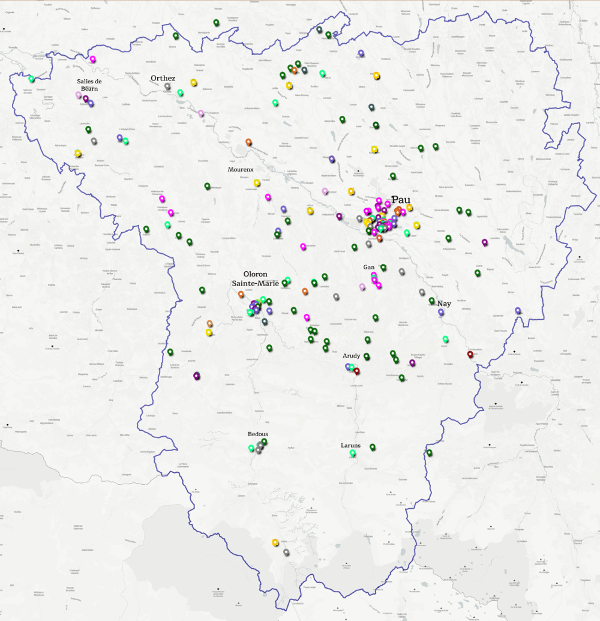
\includegraphics[width=0.9\linewidth]{carte.png}
  \end{center}
\end{multicols}


    \vspace{.5cm}

\noindent Personne n’est parfait, ni même les prestataires de la T!nda ! Mais tous ceux que nous agréons sont déjà engagés
d’une façon ou d’une autre dans la transition écologique et sociale qui fera du Béarn un endroit où il fait bon (et
encore mieux) vivre !
    \vspace{.2cm}

\noindent La Tinda vise à expérimenter un changement lent et fondamental dont chacunE peut être acteur ou actrice.

    \vspace{1cm}

      \textbf{Contact :}
    \begin{itemize}
      \item[] Particuliers : \href{mailto:contact@demainenmain.org}{contact@demainenmain.org}
      \item[] Professionnels : \href{mailto:prestataires@demainenmain.org}{prestataires@demainenmain.org}
      \item[] Mobile : 07 83 29 30 53 
      \item[] Site web : \href{https://www.demainenmain.org}{www.demainenmain.org}
    \end{itemize}

    \vspace{1cm}

  \begin{center}
    {\Large \textbf{Adhérez à De Main En Main et échanger des € contre des T! dans les comptoirs d’échanges !!}}
  \end{center}

\pagebreak

  \begin{center}
\input{presta_zip_comptoir.tex}

\pagebreak

    {\Large Les prestataires du réseau par ordre alphabétique}
    \begin{longtable}{|m{\nameWidth} | m{\dataWidth}|}
      \hline
      Nom & Coordonnées  \\ 
      \hline 
      \endhead

      \input{presta_zip_alpha.tex}
    \end{longtable}
  \end{center}
\end{document}
